% Options for packages loaded elsewhere
\PassOptionsToPackage{unicode}{hyperref}
\PassOptionsToPackage{hyphens}{url}
%
\documentclass[
]{article}
\usepackage{amsmath,amssymb}
\usepackage{iftex}
\ifPDFTeX
  \usepackage[T1]{fontenc}
  \usepackage[utf8]{inputenc}
  \usepackage{textcomp} % provide euro and other symbols
\else % if luatex or xetex
  \usepackage{unicode-math} % this also loads fontspec
  \defaultfontfeatures{Scale=MatchLowercase}
  \defaultfontfeatures[\rmfamily]{Ligatures=TeX,Scale=1}
\fi
\usepackage{lmodern}
\ifPDFTeX\else
  % xetex/luatex font selection
\fi
% Use upquote if available, for straight quotes in verbatim environments
\IfFileExists{upquote.sty}{\usepackage{upquote}}{}
\IfFileExists{microtype.sty}{% use microtype if available
  \usepackage[]{microtype}
  \UseMicrotypeSet[protrusion]{basicmath} % disable protrusion for tt fonts
}{}
\makeatletter
\@ifundefined{KOMAClassName}{% if non-KOMA class
  \IfFileExists{parskip.sty}{%
    \usepackage{parskip}
  }{% else
    \setlength{\parindent}{0pt}
    \setlength{\parskip}{6pt plus 2pt minus 1pt}}
}{% if KOMA class
  \KOMAoptions{parskip=half}}
\makeatother
\usepackage{xcolor}
\usepackage[margin=1in]{geometry}
\usepackage{longtable,booktabs,array}
\usepackage{calc} % for calculating minipage widths
% Correct order of tables after \paragraph or \subparagraph
\usepackage{etoolbox}
\makeatletter
\patchcmd\longtable{\par}{\if@noskipsec\mbox{}\fi\par}{}{}
\makeatother
% Allow footnotes in longtable head/foot
\IfFileExists{footnotehyper.sty}{\usepackage{footnotehyper}}{\usepackage{footnote}}
\makesavenoteenv{longtable}
\usepackage{graphicx}
\makeatletter
\def\maxwidth{\ifdim\Gin@nat@width>\linewidth\linewidth\else\Gin@nat@width\fi}
\def\maxheight{\ifdim\Gin@nat@height>\textheight\textheight\else\Gin@nat@height\fi}
\makeatother
% Scale images if necessary, so that they will not overflow the page
% margins by default, and it is still possible to overwrite the defaults
% using explicit options in \includegraphics[width, height, ...]{}
\setkeys{Gin}{width=\maxwidth,height=\maxheight,keepaspectratio}
% Set default figure placement to htbp
\makeatletter
\def\fps@figure{htbp}
\makeatother
\setlength{\emergencystretch}{3em} % prevent overfull lines
\providecommand{\tightlist}{%
  \setlength{\itemsep}{0pt}\setlength{\parskip}{0pt}}
\setcounter{secnumdepth}{5}
\newlength{\cslhangindent}
\setlength{\cslhangindent}{1.5em}
\newlength{\csllabelwidth}
\setlength{\csllabelwidth}{3em}
\newlength{\cslentryspacingunit} % times entry-spacing
\setlength{\cslentryspacingunit}{\parskip}
\newenvironment{CSLReferences}[2] % #1 hanging-ident, #2 entry spacing
 {% don't indent paragraphs
  \setlength{\parindent}{0pt}
  % turn on hanging indent if param 1 is 1
  \ifodd #1
  \let\oldpar\par
  \def\par{\hangindent=\cslhangindent\oldpar}
  \fi
  % set entry spacing
  \setlength{\parskip}{#2\cslentryspacingunit}
 }%
 {}
\usepackage{calc}
\newcommand{\CSLBlock}[1]{#1\hfill\break}
\newcommand{\CSLLeftMargin}[1]{\parbox[t]{\csllabelwidth}{#1}}
\newcommand{\CSLRightInline}[1]{\parbox[t]{\linewidth - \csllabelwidth}{#1}\break}
\newcommand{\CSLIndent}[1]{\hspace{\cslhangindent}#1}
\newcommand{\beginappendix}{ \setcounter{table}{0} \renewcommand{\thetable}{A\arabic{table}} \setcounter{figure}{0} \renewcommand{\thefigure}{A\arabic{figure}} }
\usepackage[capposition=top]{floatrow}
\usepackage{placeins}
\usepackage{setspace}
\usepackage{dcolumn}
\usepackage{booktabs}
\usepackage{siunitx}
\usepackage{amsmath}
\usepackage{enumerate}
\usepackage[shortlabels]{enumitem}
\usepackage[hang,flushmargin]{footmisc}
\usepackage{makecell}
\usepackage{booktabs}
\usepackage{longtable}
\usepackage{array}
\usepackage{multirow}
\usepackage{wrapfig}
\usepackage{float}
\usepackage{colortbl}
\usepackage{pdflscape}
\usepackage{tabu}
\usepackage{threeparttable}
\usepackage{threeparttablex}
\usepackage[normalem]{ulem}
\usepackage{makecell}
\usepackage{xcolor}
\ifLuaTeX
  \usepackage{selnolig}  % disable illegal ligatures
\fi
\IfFileExists{bookmark.sty}{\usepackage{bookmark}}{\usepackage{hyperref}}
\IfFileExists{xurl.sty}{\usepackage{xurl}}{} % add URL line breaks if available
\urlstyle{same}
\hypersetup{
  pdftitle={Air pollution and agricultural productivity in a developing country},
  pdfauthor={Joshua D. Merfeld},
  hidelinks,
  pdfcreator={LaTeX via pandoc}}

\title{Air pollution and agricultural productivity in a developing country\footnote{I thank Ariel Ortiz-Bobea, Marc Bellemare, and David Sungho Park for comments and suggestions that greatly improved the quality of the paper, as well as conference attendees at the 2023 KER International Conference and the University of Reading. The usual disclaimer applies. All scripts used in this paper are publicly available on my GitHub page: github.com/JoshMerfeld/pollution\_development}}
\author{Joshua D. Merfeld\footnote{KDI School of Public Policy and Management and IZA; \href{mailto:merfeld@kdis.ac.kr}{\nolinkurl{merfeld@kdis.ac.kr}}}}
\date{2023-07-19}

\begin{document}
\maketitle
\begin{abstract}
\noindent I document negative externalities of air pollution in the Indian agricultural sector. Using variation in pollution induced by changes in wind across years, I show that higher levels of pollution lead to decreased agricultural productivity. The negative effects of pollution are larger in areas growing more labor-intensive crops, indicating that the pollution works partly through direct effects on labor productivity. I also show that pollution from coal plants has a larger effect on agricultural productivity than other types of pollution. These results suggest that the negative externalities of pollution may hit the poorest particularly hard, given their reliance on agriculture.\\
\strut \\
\textbf{\textit{Keywords}}: pollution, productivity, agriculture, labor, India\\
\textbf{\textit{JEL Codes}}: H40, I15, J22, O13, Q52, Q53
\end{abstract}

\newpage
\doublespacing

\hypertarget{introduction}{%
\section{Introduction}\label{introduction}}

In 2021, energy generation from coal reached an all-time high,\footnote{www.iea.org/reports/coal-fired-electricity} driven in part by rapid population growth in developing countries, including India. While natural gas has become a popular alternative in much of the world, the Indian government met much of the increased demand through the construction of coal power plants. From 1990 to 2010, India's population grew by more than 40 percent, leading to a large increase in demand for power.\footnote{data.worldbank.org} During those same two decades, power generation from all coal units of at least 30 megawatts in the country more than doubled, from 42.4 gigawatts to more than 100 gigawatts.\footnote{globalenergymonitor.org/}

While electricity may lead to economic and productivity growth (Dinkelman 2011; Kline and Moretti 2014; Rud 2012; Van de Walle et al. 2017), though electrification alone may not be a sufficient condition (K. Lee, Miguel, and Wolfram 2020), these improvements do not come without downsides, especially when it comes to power derived from coal. Emissions from the production and burning of coal -- pollutants like sulfur dioxide, nitrogen oxides, methane, and mercury, for example -- are also directly harmful to human health and the environment. Although the use of coal had been declining, recent events -- including Russia's invasion of Ukraine -- have led to an increase in the demand for coal.\footnote{www.npr.org/2022/08/15/1117560560/a-rising-demand-for-coal-amidst-war-in-ukraine}

Pollution more generally is also increasing in much of the world. Carbon dioxide equivalent per capita has almost doubled over the last 50 years in India, more than doubled in Indonesia, and almost tripled in China.\footnote{\url{https://edgar.jrc.ec.europa.eu}} Much of this increase is due to the development process itself -- as countries develop, their economies transform, with more people moving out of agriculture and into manufacturing and services (Herrendorf, Rogerson, and Valentinyi 2014). Despite this development, agriculture remains a key sector in many developing countries, employing a large proportion of the poor (Dercon 2009), and agriculture is a key sector for poverty reduction (Christiaensen, Demery, and Kuhl 2011). This raises an important question: do rising pollution levels in developing countries threaten agricultural productivity?

In this paper, I study the effects of pollution on agricultural productivity in India. Previous work has suggested that there may be harmful direct effects of air pollution (Heck et al. 1982; Marshall et al. 1997) and water pollution (Reddy and Behera 2006) on agricultural productivity, including work showing that gold mines -- which release large amounts of pollutants into the surrounding environment -- lead to lower agricultural productivity in Ghana (Aragón and Rud 2016). These effects can work through the well-known effects on human health and productivity, but also directly through land productivity. Black carbon in soot, for example, can directly affect solar radiation reaching plants on the surface (Ramanathan and Carmichael 2008; Burney and Ramanathan 2014), while, on the other hand, sulfur in some pollution sources can actually be productivity enhancing (Sanders and Barreca 2022). Relative to previous work in economics, this paper tackles pollution more broadly, before turning to a specific source of pollution: coal plants. I show that air pollution leads to lower agricultural productivity in India and that pollution from coal plants is particularly harmful to agriculture.

Identifying the causal effects of pollution is difficult. For starters, the construction of coal plants is likely to be endogenous, though the relationship between construction and economic conditions is not a priori clear. On the one hand, governments may locate new plants in fast-growing areas, while on the other hand, they may decide the exact location of plants based on the political power of local citizens (Kopas et al. 2020). In the case of the data I use here, coal plants are constructed in areas with higher population and higher levels of pollution. In terms of agriculture, higher productivity predicts more coal plants in a given year as well as the construction of a coal plant over the next decade, indicating possible bias when estimating effects of pollution on agricultural productivity.

To identify the effects of air pollution on agricultural productivity, I identify areas of high pollution emission using the location of coal plants. While coal plants may add emissions, I show that they are located in areas with relatively higher levels of pollution, in general. Using these locations as point sources of pollution, I use plausibly exogenous changes in wind direction -- in a similar spirit to Deryugina et al. (2019) -- to measure the effects of pollution on key agricultural outcomes. I first plot the location of coal plants in India by year. Using a village-level shapefile, I identify all villages that are located within 30km of a coal plant at any time during the sample period, which comprises the 2000s to the 2010s, with differences across outcomes depending on data availability. I then calculate the direction from each coal plant to all villages within 30km. I include all areas, regardless of whether the coal plant has opened yet, to allow me to disaggregate the effects of pollution from coal plants with other kinds of pollution later in the paper.

Using daily wind data and these spatial variables, I create an identifier separately for every village for whether a given village is located downwind from a coal plant on any given day. I then aggregate this exposure variable based on the desired analysis; for agricultural productivity, for example, I create an exposure variable measuring the total number of exposure days in the five-month agricultural season, focusing only on the monsoon (Kharif) season. More days being located downwind from a high-pollution location leads to substantially higher average concentrations of particulate matter 2.5 (PM 2.5), which is defined as particulate matter with a diameter of less than 2.5 micrometers.

Using wind direction as an instrument for particulate matter, an increase of PM 2.5 by one percent leads to a large decrease in agricultural productivity, with an elasticity of approximately -0.63 in the most conservative specification. The IV estimates indicate that the effect of pollution is more negative than naïve OLS estimates, which is consistent with the evidence on the construction of coal plants; higher levels of pollution are correlated with higher levels of agricultural productivity, a relationship that the IV strategy adjusts downwards. Robustness checks confirm these main results. Randomization inference shows that the estimates are robust to alternative measures of uncertainty, while leads of pollution do not affect current agricultural productivity.

Heterogeneity analysis shows that the negative effects of pollution are larger in villages that experience higher median exposure to pollution and in villages with higher initial yields. Finally, given how many poor farmers rely on rainfall and how weather shocks are on the rise across the globe, I also look at possible multiplicative effects of shocks by interacting the pollution variables with a rainfall variable. Higher exposure along with less rainfall increases the negative effect of either shock individually, meaning these shocks are compounding. Given concerns regarding agricultural productivity and climate change, the rise of pollution in India may be particularly problematic for poor farmers.

A key question is the mechanism: does pollution reduce labor productivity, land productivity, or both? While previous work from the United States indicates that pollution from coal plants, specifically, can lead to higher \emph{land} productivity (Sanders and Barreca 2022), agriculture in India differs greatly from agriculture in the United States. To test for possible effects on labor productivity, I look at differential effects based on labor intensity of the predominant crops in different villages. Specifically, I separate effects in predominantly rice-growing areas from other areas; since rice is very labor intensive, we would expect to see larger negative effects of pollution in rice-growing regions relative to other regions if one mechanism through which pollution affects productivity is direct effects on labor. I show that pollution negatively effects agricultural productivity in non-rice areas but that the effects in rice-growing areas are around 50 percent larger in magnitude. These results indicate that pollution likely directly affects labor productivity, though I am not able to rule out direct effects on land, either, due to a lack of data.

The final set of analyses disentangles the effects of pollution from the effects of coal pollution, specifically, by using wind direction and the rollout of coal plants across the country. Combining instrumental variables with a differences-in-differences strategy, I show that agricultural productivity has an elasticity of around -0.22 with respect to non-coal pollution. The opening of a coal plant, however, doubles the elasticity, to more than -0.44, indicating that coal plant emissions are particularly harmful to agricultural productivity, at least in India. This is consistent with coal emissions being quite different from other forms of pollution; coal emissions contain different types and quantities of harmful substances, meaning effects may differ greatly.

An important caveat to these results is that I cannot disentangle exactly which pollutants drive results. While I use PM 2.5 as a measure of overall exposure to pollution, effects could be driven by any pollutants carried by the wind. This leaves open an important avenue of future research regarding the effects of different types of pollutants on agricultural productivity.

The results are consistent with evidence of effects of pollution on different forms of labor activity. For example, general levels of pollution decrease productivity of call center works in China (Chang et al. 2019), lead people to perform worse on cognitive functions (Ebenstein, Lavy, and Roth 2016; Wen and Burke 2022), lower labor market earnings (Borgschulte, Molitor, and Zou 2022), and also lead to lower levels of farm labor productivity in California, driven by changes in ozone concentration (Graff Zivin and Neidell 2012). Also in China, He, Liu, and Salvo (2019) find small but significant negative effects of pollution on manufacturing productivity, while Chen, Oliva, and Zhang (2022) show pollution leads to labor out migration. Relevant to my results, Hanna and Oliva (2015) show that decreases in pollution lead to increases in labor allocation in Mexico.

Several papers are closely related to this one. Aragón and Rud (2016) show that gold mines in Ghana have substantial negative impacts on agricultural productivity in the surrounding areas. Burney and Ramanathan (2014) model the effects of climate change and pollutants on agricultural productivity in India. Finally, Sanders and Barreca (2022) actually find that coal emissions can be good for agriculture in the United States, due to the presence of sulfur, which can increase agricultural productivity. This paper differs from the previous literature in three important ways. First, I explore effects of pollution more generally as well as from coal plants, which are much more ubiquitous than gold mines across the world. Second, I use a different identification strategy from most other papers, relying on wind blowing pollution from coal plants. Finally, agriculture in India and the United States can be quite different, with the latter being much more mechanized. This means effects of pollution could differ substantially depending on the context, a conclusion that the current results support.

\hypertarget{data}{%
\section{Data}\label{data}}

\label{data}

The main goal of this paper is to examine whether exposure to pollution affects agricultural productivity, as well as to provide evidence about the effects of pollution from coal plants, in particular. I use several sources of data, which I describe here and list in Table \ref{tab:data} of the appendix.

The first set of data lists the location of coal plant across the globe. This data comes from Global Energy Monitor\footnote{globalenergymonitor.org/projects/global-coal-plant-tracker/} and lists all units generating at least 30 megawatts of electricity. The data on coal plants includes the year of opening (and, if applicable, the year of retirement), the GPS (latitude/longitude) location of each plant, and the amount of power produced by the units at each plant. For this paper, I do not use the information on the capacity of the plant.

Figure \ref{fig:plants} in the appendix displays the location of coal plants in India for two specific years: 1990 and 2010. There is a clear increase in the prevalence of coal plants across the country over the two decades. Additionally, the overall capacity from coal plants increased from 42.4 gigawatts to 100.4 gigawatts, an increase of 136.6 percent in just 20 years. This increase is driven both by the roll out of new plants as well as the construction of new units at existing plants, the latter of which is not shown in Figure \ref{fig:plants}.

The second dataset includes agricultural productivity for both the monsoon and winter seasons, from 2002 to 2018. To match other data, I only use the data up to 2013. This data comes from Gangopadhyay et al. (2022) and estimates land productivity (i.e.~yield, in tons per hectare) for the major crops in India, using satellite-derived data. While there is a wealth of literature on measurement error in land (Desiere and Jolliffe 2018; Abay et al. 2022), the authors use a static cropland mask for the productivity estimates. This means that any measurement error will hopefully be constant across time and subsumed by the village fixed effects. While the measure of output is also noisy, the use of satellite-derived data and a static cropland mask reduces concerns about measurement error being responsible for the results below, especially since common sources of measurement error are unlikely to be correlated with wind direction. The authors define the monsoon season as June to October and the winter season as November to March. Due to large differences in the crops grown and the production technologies used across seasons, I focus on only the monsoon season and keep the authors' definition when matching across data below. The data on agricultural productivity is publicly available from Nature's data-sharing website.\footnote{springernature.figshare.com} Since the main regressions below use village fixed effects, any differences in cropping patterns across areas should not bias estimates on changes, as long as these patterns do not change markedly in response to annual pollution levels.

The agricultural productivity data is available as raster files with a resolution of 500m. To aggregate this data up to a useful administrative unit, I use village-level shapefiles provided by Asher et al. (2021) and publicly available on the SHRUG platform.\footnote{www.devdatalab.org/shrug\_download/} I aggregate the agricultural productivity data to the village level by extracting mean productivity for each feature in the shapefile. I do this separately for the monsoon season each year, from 2002 to 2013.

To measure exposure to pollution from point sources around coal plants, I first locate all village centroids located within 30km from a coal plant in a given year. I choose 30km due to previous research on the effects of (air) pollution (Aragón and Rud 2016; Bencko and Symon 1977; Li and Gibson 2014). I then calculate the direction from these point sources to all village centroids within that 30km radius. To define exposure, I pull daily wind direction data from the National Center for Atmospheric Research.\footnote{climatedataguide.ucar.edu/} For each day, I document whether the wind is blowing towards each village centroid\footnote{I define ``towards'' as within five degrees to help take into account that I am using village centroids. The wind data includes both the x and y components of wind speed, which I can use to calculate angles from point sources to village centroids.} and then temporally aggregate this daily data depending on the temporal definition of the corresponding outcome. For example, agricultural productivity is defined across five months (i.e.~the monsoon season is from June to October) so I count the total days a given village is exposed to wind blowing from \emph{any} coal plant within 30km during those five months.

The top panel in Figure \ref{fig:windexample} in the appendix is an example wind direction raster. The raster shows wind direction for the entirety of India on January 1st, 2010, as well as the location of coal power plants on that date. The prevailing winds on the date differ across the country and, though not shown in the figure, across days. This means that the overall exposure for a given area to coal plant emissions changes across time.

For pollution data, I use estimated particulate matter (PM). Specifically, I use estimates of PM 2.5, which includes particles with a diameter of 2.5 micrometers or less. This data comes from Hammer et al. (2020) and is available as a raster with a resolution of 0.01 degrees. I aggregate this data to the village level by extracting the mean PM for each feature in the shapefile. I do this separately for each month from June 2002 to October 2013. The bottom panel in Figure \ref{fig:windexample} in the appendix is an example of the PM data. The figure shows the estimated PM 2.5 from for each village in Guna district of Madhya Pradesh on January 1st, 2010.

While I use PM 2.5 as the estimated level of pollution, it is important to clarify that I cannot explicitly say that PM 2.5, per se, is responsible for any effects. Pollution includes a variety of different components, including PM 2.5, PM 10, sulfur dioxide, and nitrogen dioxide, to name but a few. While I use PM 2.5 as a proxy for pollution, it is possible that other components are responsible for the effects. Additionally, the PM 2.5 data is estimated using satellite data and a machine learning algorithm. While this is a common approach in the literature ( see Hammer et al. (2020) for more details), it is important to note that the estimates are not direct measurements of pollution. However, a valid instrumental variable can help for any measurement error present in the data (Glewwe 2012; Gillen, Snowberg, and Yariv 2019).

To help understand some of the mechanisms driving the relationship between exposure to emissions and agricultural productivity, I also look at the differential effects by the labor intensity of the predominant crop in each area. For this, I use data from Monfreda, Ramankutty, and Foley (2008), who estimate area harvested for different crops across the global around the year 2000. I identify areas where rice (paddy) is the most commonly grown crop, under the assumption that rice is more labor intensive than other crops (Vollrath 2011; Michler 2020). Michler (2020), for example, shows that rice, on avearge, uses almost 1,800 hours per hectare, while the second-highest crop in his data, cotton, juses just 850. He also estimates that wheat, another common crop in India, uses just 600 hours per hectare.

\hypertarget{methods}{%
\section{Methods}\label{methods}}

\label{identification}

I am primarily interested in the effects of pollution on agricultural productivity. We might consider a regression of the following form:
\begin{gather} y_{it} = \alpha_{i} + \gamma_{t} + \beta PM_{it} + \delta rain_{it} + \psi temp_{it} + \varepsilon_{it}, \end{gather}

where \(y_{it}\) is outcome \(y\) for unit \(i\) at time \(t\), \(\alpha\) is a geographic fixed effects, \(\gamma_t\) is time fixed effects, \(PM_{it}\) is the (log) concentration of particulate matter 2.5, \(rain_{it}\) is total rainfall during the season, and \(temp_{it}\) is average temperature during the season.

However, even with the fixed effects, this regression likely suffers from endogeneity; places with more pollution may be very different from places with less pollution. It is difficult to sign the direction of the bias a priori, because it depends on the local context and how the coal plants are placed. For example, if coal plants are placed in places in need of power -- for example, due to rapid growth -- then the estimates might be upwards biased. On the other hand, if officials purposefully place coal plants in poorer areas for political reasons, then the estimates might be downwards biased.

What are the characteristics of areas near the construction of new coal plants? Table \ref{tab:plantresultstable} presents four separate regressions, using state-level fixed effects due to the spatial variation in coal plants. The first two columns use 1991 census data -- downloaded from SHRUG -- and the second two columns use 2001 census data, all at the village level. The first column presents results from regressing a dummy for whether there is a coal plant within 30km in 1991 on several census variables. Villages with higher population densities (higher log population and lower log area) are more likely to be near a coal plant at the time. Urban population proportion is not a significant predictor after conditioning on population and area.

\begin{table}

\caption{\label{tab:plantresultstable}Local characteristics and the construction of coal plants}
\centering
\begin{threeparttable}
\begin{tabular}[t]{>{\raggedright\arraybackslash}p{3.5cm}>{\centering\arraybackslash}p{2cm}>{\centering\arraybackslash}p{2cm}>{\centering\arraybackslash}p{2cm}>{\centering\arraybackslash}p{2cm}}
\toprule
\multicolumn{1}{c}{ } & \multicolumn{2}{c}{1991 census} & \multicolumn{2}{c}{2001 census} \\
\cmidrule(l{3pt}r{3pt}){2-3} \cmidrule(l{3pt}r{3pt}){4-5}
  & 1991 & 2001 & 2001 & 2011\\
\midrule
Population (log) & 0.012*** & 0.009*** & 0.015*** & 0.006***\\
 & (0.001) & (0.000) & (0.000) & \vphantom{1} (0.000)\\
Area (log) & -0.010*** & -0.005*** & -0.010*** & -0.005***\\
 & (0.001) & (0.000) & (0.000) & (0.000)\\
Urban pop (prop) & -0.029 & 0.006 & -0.003 & -0.007\\
 & (0.037) & (0.035) & (0.022) & (0.018)\\
Ag. productivity &  &  & 0.014*** & 0.028***\\
 &  &  & (0.001) & (0.001)\\
Pollution (log PM 2.5) &  &  & 0.051*** & 0.016***\\
 &  &  & (0.002) & (0.001)\\
Sub-sample & all & no plant & all & no plant\\
\midrule
Observations & 283,021 & 264,265 & 508,786 & 469,005\\
\bottomrule
\end{tabular}
\begin{tablenotes}[para]
\item Note: State fixed effects are included in regressions. Robust standard errors are in parentheses. The outcome in the first column is whether the village is within 30km of a coal plant in 1991. The second column is whether a village in 1991 will have a coal plant in 2001, conditional on not having one in 1991. The last two columns are similarly defined, except using 2001 and 2011 as the years. * p<0.10 ** p<0.05 *** p<0.01
\end{tablenotes}
\end{threeparttable}
\end{table}

The second column keeps the 1991 census data but changes the outcome variable to a dummy for whether there \emph{will be} a coal plant constructed within 30km before 2001. This column restricts the sample to only villages that do not already have a coal plant within 30km in 1991. The pattern of significance remains the same in column two.

The last two columns are particularly relevant to the current results. They present similar results to those in the first two columns, but use the 2001 census data and a dummy for the presence of a coal plant in 2001 and 2011 in columns three and four, respectively. Importantly, I include agricultural productivity in the monsoon season of 2002 -- the earliest year available -- as well as average pollution during the monsoon season for 1998 through 2000 as additional predictors. In 2001, agricultural productivity is a strong predictor for the presence of a coal plant. Moreover, it is also a significant predictor of the construction of a coal plant between 2001 and 2011 (column four). Given that the coefficient is positive, this indicates that coal plants are more likely to be built in areas with higher agricultural productivity. In other words, any selection in the overall location of coal plants would bias against finding negative effects of pollution on agricultural productivity. However, note that this is not the same as looking at wind direction, though comparing the OLS and IV results below leads to the same conclusion regarding selection.

Pollution is also a significant predictor for the presence of a coal plant in 2001 as well as for whether a coal plant will be constructed before 2011. While the coefficient is relatively small, it is actually quite large given that only three percent of villages in column four will get a new plant in the next decade.

Since pollution is likely to be endogenous, a naïve OLS regression will not return unbiased estimates. The experimental ideal would be to randomly assign pollution to villages, but this is obviously not possible. Instead, I use an instrumental variables (IV) approach to identify the causal effects of pollution on agricultural productivity. The key identifying assumption is that wind direction is exogenous from year to year, conditional on village fixed effects and weather. While the location of pollution sources might be endogenous, the amount of pollution received by a specific village in a given year can vary randomly based on wind direction. By counting the number of days in a given year that a village is downwind from a polluted area and conditioning on village fixed effects and weather (rainfall and temperature), variation across years is plausibly exogenous. Since I include village fixed effects, identification comes from within-village changes in wind direction across years.

Consider the reduced form effect of wind exposure on agricultural productivity:
\begin{gather} PM2.5_{it} = \alpha_{i} + \gamma_{t} + \beta wind_{it} + \delta rain_{it} + \psi temp_{it} + \varepsilon_{it}, \end{gather}

where variables are defined identically to above but with wind as the primary variable of interest instead of pollution. Combining these into a two-stage procedure, we can instrument for pollution using wind direction; small changes in wind direction can lead to large changes in pollution exposure for villages located near point sources of pollution, allowing me to identify the causal effects of pollution by isolating the random component driven by wind direction. This is similar in spirit to Deryugina et al. (2019).

Identification relies on changes in wind direction across time for the same geographic units. In other words, conditional on the fixed effects and weather, I assume changes in wind direction are as good as random and uncorrelated with the outcome -- primarily agricultural productivity in this paper -- except through exposure to pollution.

The inclusion of rainfall and temperature is meant to reduce concerns that wind direction may not affect agricultural productivity but, instead, be correlated with it through changes in weather. For example, prevailing winds from one direction may be associated with dry weather, while winds from another direction may be more likely to carry moisture and rain. It is not a priori clear how this would bias the estimates with respect to pollution and coal plants, however. The differences in weather patterns is very context specific and can differ even for villages located near one another.

I believe there are two reasons this is unlikely to be the case here. First, villages located near one another have very similar weather patterns, but wind direction leads to large differences in pollution exposure even for villages right next to one another. Second, in some specifications, I include very flexible specifications for weather. These inclusions do not lead to very large changes in the estimated relationship between pollution and agricultural productivity, suggesting that weather is unlikely to be responsible for a spurious correlation between productivity and pollution in the main results.

It is worth taking the time to validate the use of wind direction as a measure of exposure to pollution. Consider the data used for the regressions presented in Table \ref{tab:yield3ivmainfirststage} of the appendix. The outcome variable is particulate matter -- specifically, \(\mathrm{PM 2.5}\), which is particulate matter no larger than 2.5 micrometers in diameter -- which comes from Hammer et al. (2020). \(\mathrm{PM 2.5}\) is one of the harmful byproducts from many industrial processes, including power generation. Particulate matter is a major component of the pollution emitted by coal plants, along with sulfur dioxide, different types of nitrogen oxides, and mercury.\footnote{www.epa.gov/airmarkets/power-plants-and-neighboring-communities} This data is available at the monthly level, but I aggregate variables to the season variable since that is the level of analysis in the main results.

Both the particulate matter data and the wind data is at the village level, which means the regressions in Table \ref{tab:yield3ivmainfirststage} are at the village level. As such, the geographic fixed effects are village fixed effects and the temporal fixed effects are month fixed effects. Since the exposure variable is at the village level and we follow villages over time, the standard errors are also clustered at the village level. I add more and more flexible specifications for weather, with the most flexible specification in the fourth column. Note that the relationship between wind direction and particulate matter is very similar across all four columns, suggesting that the inclusion of weather does not change the relationship between wind direction and pollution. This is important because it suggests that the use of wind direction as a proxy for pollution exposure is not biased by weather patterns.

\hypertarget{identifying-mechanisms}{%
\subsection{Identifying mechanisms}\label{identifying-mechanisms}}

A key question is how pollution affects agricultural productivity. Specifically, does pollution directly affect labor productivity, land productivity, or both? Unfortunately, there is a lack of data that would allow me to directly test these mechanisms, since I do not have data on the amount of labor or land used in each village. Instead, I look at heterogeneity in the effects of pollution based on the predominant crop grown in each village.

Michler (2020) presents estimates of labor intensity for several major crops in India. The most labor-intensive crop is rice, which uses almost 1,800 hours per hectare. The second-most labor-intensive crop is cotton, which uses just 850 hours per hectare. Wheat, another common crop in India, uses just 600 hours per hectare. This suggests that pollution should be more harmful for rice than for other crops if there are direct impacts on labor productivity.

To identify this possible mechanism, I identify areas that grow predominantly rice. Specifically, I estimate the following regression:
\begin{gather} 
y_{it} = \alpha_{i} + \gamma_{t} + \omega PM_{it} + \phi rice_{it} + \beta PM_{it}\times rice_{it} + \delta rain_{it} + \psi temp_{it} + \varepsilon_{it},
\end{gather}
where \(PM_{it}\) denotes the effect of pollution in non-rice areas and \(PM_{it}\times rice_{it}\) is the differential effect in rice-growing areas. Here, I create an indicator variable for rice areas that is time invariant, so \(rice_{it}\) drops out of the estimation. I instrument for \(PM_{it}\) and for \(PM_{it}\times rice_{it}\) using wind and wind interacted with the indicator for rice.

While this is a useful first step, it is not a perfect identification strategy. First, there could be other differences in the types of areas that grow rice, and these differences could actually be responsible for any heterogeneity. Second, this strategy does not allow me to say anything about the effects of pollution on land productivity.

\hypertarget{identifying-effects-of-pollution-from-coal-plants}{%
\subsection{Identifying effects of pollution from coal plants}\label{identifying-effects-of-pollution-from-coal-plants}}

I use the location of coal plants to identify locations of high pollution emission, but there can be other pollution sources located near coal plants, as well. I nonetheless also want to identify the effects of pollution coming specifically from coal plants, in addition to the overall effects of pollution in the other parts of the paper. I do this by combining the two-stage procedure above with a differences-in-differences framework. Specifically, I create a new variable identifying the exact year the coal plant opens in a given area and calculate the change in the effects of pollution on agricultural productivity.

Consider the following regression of interest:
\begin{gather} 
y_{it} = \alpha_{i} + \gamma_{t} + \omega PM_{it} + \phi open_{it} + \beta PM_{it}\times open_{it} + \delta rain_{it} + \psi temp_{it} + \varepsilon_{it},
\end{gather}

where the interaction term \(PM_{it}\times open_{it}\) indicates the change in the effect of pollution following the opening of the coal plant. Note that this is not the same as saying that pollution increased; instead, it is focusing on the change in the effect of a change in pollution of one unit on the outcome of interest, agricultural yield. I instrument for both \(PM_{it}\) and \(PM_{it}\times open_{it}\) using wind and the interaction between wind and the open indicator, or \(wind_{it}\times open_{it}\).

\hypertarget{results}{%
\section{Results}\label{results}}

\label{results}

I first present the reduced form results for agricultural productivity. The outcome for all regressions in this section is the log of agricultural land productivity, which is defined as tons per hectare. The first set of results are in Table \ref{tab:yieldtable}. The unit of analysis is the village-season -- from 2002 to 2013 -- focusing only on the monsoon (kharif) season. The data used to construct the yield measure is calculated using five months of data, so the wind variable is defined for the same five months and is the sum of days in which the wind is pointed towards the village centroid from a coal plant.

The first column presents the most simple results, with only the wind exposure variable and the fixed effects. The second column adds a rainfall and average temperature variable. While I leave them out of the table for simplicity, the coefficients are in the expected direction: rainfall is positive and average temperature is negative. The third column adds higher-order weather variables for both rainfall and temperature, as well as the interaction between them. This attenuates the relationship between wind and productivity somewhat, but the coefficient remains negative and statistically significant.

The final column includes the most flexible form for the weather variables. The z-score for rainfall is turned into bins -- with cutoffs at \(z=-1\) and \(z=1\) -- based on rainfall in each month of the season. In other words, over the five months, I create 15 different indicator variables for rainfall based on the z-score in each month. One of these indicators drops out for each month of the year, leaving 10. I also include interactions between all of these and temperature, as well as between the bins and temperature squared. The coefficient on wind remains negative and statistically significant, and is actually slightly larger in magnitude than the results in column three, which is a much less flexible specification for weather. This leads me to conclude that the results are not being driven by weather patterns.

\begin{table}

\caption{\label{tab:yieldtable}Wind direction and agricultural productivity}
\centering
\begin{threeparttable}
\begin{tabular}[t]{>{\raggedright\arraybackslash}p{4cm}>{\centering\arraybackslash}p{2.5cm}>{\centering\arraybackslash}p{2.5cm}>{\centering\arraybackslash}p{2.5cm}c}
\toprule
  & (1) & (2) & (3) & (4)\\
\midrule
wind days & -0.0078*** & -0.0065*** & -0.0051*** & -0.0053***\\
 & (0.0007) & (0.0007) & (0.0007) & (0.0007)\\
weather & No & Yes & Yes & No\\
weather (expanded) & No & No & Yes & No\\
weather (expanded, bins) & No & No & No & Yes\\
\textbf{fixed effects:} & \textbf{} & \textbf{} & \textbf{} & \textbf{}\\
village & Yes & Yes & Yes & Yes\\
year & Yes & Yes & Yes & Yes\\
\midrule
observations & 1,266,922 & 1,266,922 & 1,266,922 & 1,266,922\\
\bottomrule
\end{tabular}
\begin{tablenotes}[para]
\item Note: Standard errors are in parentheses and are clustered at the village level. The outcome in all regressions is estimated agricultural yield, defined as tons per hectare. * p<0.10 ** p<0.05 *** p<0.01
\end{tablenotes}
\end{threeparttable}
\end{table}

To put the size of the coefficient in context, it is worth digging a little deeper into the exposure variable. The mean within-village absolute deviation in wind exposure is approximately 2.42 days, meaning that the average change in agricultural productivity from year-to-year due to nothing but changes in wind patterns carrying particulate matter is around 1.5 percent relative to the mean. This implies that swings in agricultural productivity -- due to wind direction -- of several percent are probably quite common, since the absolute deviation includes deviations above and below the mean.

\begin{table}

\caption{\label{tab:yieldtablepm}Particulate matter (PM 2.5) and agricultural productivity}
\centering
\begin{threeparttable}
\begin{tabular}[t]{>{\raggedright\arraybackslash}p{5cm}>{\centering\arraybackslash}p{2cm}>{\centering\arraybackslash}p{2cm}>{\centering\arraybackslash}p{2cm}c}
\toprule
  & (1) & (2) & (3) & (4)\\
\midrule
Particulate matter (log PM 2.5) & -0.042*** & -0.045*** & -0.008** & -0.041***\\
 & (0.003) & (0.003) & (0.003) & (0.003)\\
Weather & No & Yes & Yes & No\\
Weather (expanded) & No & No & Yes & No\\
weather (expanded, bins) & No & No & No & Yes\\
\textbf{Fixed effects:} & \textbf{} & \textbf{} & \textbf{} & \textbf{}\\
Village & Yes & Yes & Yes & Yes\\
Year & Yes & Yes & Yes & Yes\\
\midrule
Observations & 1,266,922 & 1,266,922 & 1,266,922 & 1,266,922\\
\bottomrule
\end{tabular}
\begin{tablenotes}[para]
\item Note: Standard errors are in parentheses and are clustered at the village level. The outcome in all regressions is estimated agricultural yield, defined as tons per hectare. * p<0.10 ** p<0.05 *** p<0.01
\end{tablenotes}
\end{threeparttable}
\end{table}

Of course, it is not wind, per se, that we are interested in. Instead, we are actually interested in better understanding the effects of exposure to pollution on agricultural productivity. Table \ref{tab:yieldtablepm} presents the same regressions as Table \ref{tab:yieldtable}, with a key difference: instead of wind exposure, it uses log average concentration of \(\mathrm{PM 2.5}\) -- from Hammer et al. (2020) -- during the season as the key explanatory variable. There is again a consistent, negative relationship between particulate matter and agricultural productivity. Since both variables are logged, the coefficients are similar to elasticities, indicating that a one-percent increase in pollution leads to an approximately 0.04 percent decrease in agricultural productivity in three of the columns.

Recall, however, the results from above: coal plants were placed in places with higher average agricultural productivity. This means that the simple regressions in Table \ref{tab:yieldtablepm} might actually be biased upwards: although pollution might negatively affect productivity, pollution is higher in more productive areas due to the endogenous placement of pollution sources in the study areas. One possible way to recover the actual effect of pollution on agricultural productivity is with an instrument. If, conditional on the fixed effects and weather variables, wind direction is exogenous and only affects agricultural productivity through pollution, then it is a valid instrument for pollution.

I present these IV results in Table \ref{tab:yieldtabletwo}, with the first-stage F-statistic at the bottom. The first-stage results -- the full results are in Table \ref{tab:yield3ivmainfirststage} of the appendix -- make clear how strong of an instrument wind is; all three F-statistics are above 1,000, meeting even the higher bar for the first-stage F-test argued for by D. Lee et al. (2022).

The second-stage results first indicate that \(\mathrm{PM 2.5}\) is a very strong predictor of agricultural productivity. Using the results in column three, a one percent increase in particulate matter leads to a 0.62 percent decrease in agricultural productivity. To put this in further perspective, the mean particulate matter concentration is just short of 40 (39.68) in the monsoon sample, while the within-village absolute deviation in particulate matter is 3.98, meaning year-to-year swings of several percent in agricultural productivity due to pollution exposure alone are common.

Column four presents one last specification; it includes a much more flexible specification for weather. This is the same binned specificaiton as I describe above. The coefficient in column four shows almost not change from those in column three, again relieving some concerns that weather may not be correctly specified, leading to a spurious correlation between particulate matter and agricultural productivity.

\begin{table}

\caption{\label{tab:yieldtabletwo}Pollution and agricultural productivity, IV estimates}
\centering
\begin{threeparttable}
\begin{tabular}[t]{>{\raggedright\arraybackslash}p{4cm}>{\centering\arraybackslash}p{2cm}>{\centering\arraybackslash}p{2cm}>{\centering\arraybackslash}p{2cm}>{\centering\arraybackslash}p{2cm}}
\toprule
  & (1) & (2) & (3) & (4)\\
\midrule
Particulate matter & -0.941*** & -0.769*** & -0.621*** & -0.626***\\
(log PM 2.5) & (0.078) & (0.075) & (0.080) & (0.077)\\
Weather & No & Yes & Yes & No\\
Weather (expanded) & No & No & Yes & No\\
Weather (expanded, bins) & No & No & No & Yes\\
\textbf{Fixed effects:} & \textbf{} & \textbf{} & \textbf{} & \textbf{}\\
Village & Yes & Yes & Yes & Yes\\
Year & Yes & Yes & Yes & Yes\\
\midrule
F (first stage) & 1,236 & 1,266 & 1,205 & 1,246\\
Observations & 1,266,922 & 1,266,922 & 1,266,922 & 1,266,922\\
\bottomrule
\end{tabular}
\begin{tablenotes}[para]
\item Note: Standard errors are in parentheses and are clustered at the village level. The outcome in all regressions is estimated agricultural yield, defined as tons per hectare. * p<0.10 ** p<0.05 *** p<0.01
\end{tablenotes}
\end{threeparttable}
\end{table}

The comparison of the results to those in the previous table also confirm the concerns around endogenous placement of pollution sources. The coefficients in Table \ref{tab:yieldtabletwo} are substantially more negative than those in Table \ref{tab:yieldtablepm}. In other words, the simple regression of agricultural productivity on pollution results in coefficients on pollution that are upwards biased, since higher levels of pollution occur in more productive areas, on average. The IV strategy corrects this bias and leads to a robust, negative relationship between pollution and agricultural productivity.

\hypertarget{robustness-checks}{%
\subsection{Robustness checks}\label{robustness-checks}}

In this section, I report the results of two separate robustness checks for the main results presented above. In the previous results, standard errors are clustered at the level of the village, which is also the level at which treatment (exposure to pollution) is assigned as well as the level at which agricultural productivity is extracted. Past work has shown that standard errors might be underestimated in such contexts (Bertrand, Duflo, and Mullainathan 2004). This is a particular concern in the present case, since agricultural productivity is extracted at the village level but estimated using less coarse data that has high spatial correlation (Gangopadhyay et al. 2022).

To help remedy concerns, I perform randomization inference (e.g. Barrios et al. (2012)) by randomly assigning observed treatment across villages and repeating this process 1,000 times. I do this in two separate ways. First, I take all villages in a given year and randomly assign, with replacement, treatment intensity within the year. Second, I do this separately by selecting from within district-years only, to help take into account district-year correlation in outcomes and as a way to mitigate possible concerns that traditional clustered standard errors may actually be much too conservative (Abadie et al. 2023). Since this is an instrumental variables procedure, I randomly select the wind and pollution variable \emph{together}.

I present these results in Figure \ref{fig:randomplot} of the appendix. The purple density is the resulting distribution of estimated treatment effects when selecting from all villages within the same year. The density of treatment effects is relatively tight around 0, with the left tail only reaching slightly beyond -0.05, compared to the most conservative actual estimated treatment effect of -0.63.

The within-district correlation in outcomes and treatment is apparent when instead randomly selecting from only villages within the same district in the same year. The distribution is still approximately normal but has a mode of almost -0.4. Nonetheless, the actual treatment effect is larger in magnitude than almost all of the bootstrapped replications. The results are apparently robust to alternative specifications of uncertainty.

The second robustness check includes leads of pollution and wind direction. I instrument for future pollution using future wind direction, which mirrors the strategy employed in the main results. I present these results in Table \ref{tab:yieldtableleads}. Neither a one-year nor a two-year lead predicts current agricultural productivity, which supports the identification assumptions.

\begin{table}

\caption{\label{tab:yieldtableleads}Agricultural productivity and pollution leads}
\centering
\begin{threeparttable}
\begin{tabular}[t]{>{\raggedright\arraybackslash}p{5.5cm}>{\centering\arraybackslash}p{1.5cm}>{\centering\arraybackslash}p{1.5cm}}
\toprule
  & (1) & (2)\\
\midrule
particulate matter (one-year lead) & -0.033 & \\
 & (0.067) & \\
particulate matter (two-year lead) &  & -0.070\\
 &  & (0.052)\\
weather (expanded) & No & No\\
\textbf{fixed effects:} & \textbf{} & \textbf{}\\
village & Yes & Yes\\
year & Yes & Yes\\
\midrule
F & 592 & 783\\
observations & 1,161,265 & 1,055,562\\
\bottomrule
\end{tabular}
\begin{tablenotes}[para]
\item Note: Standard errors are in parentheses and are clustered at the village level. The outcome in all regressions estimated agricultural yield (tons per hectare). * p<0.10 ** p<0.05 *** p<0.01
\end{tablenotes}
\end{threeparttable}
\end{table}

\hypertarget{heterogeneity}{%
\subsection{Heterogeneity}\label{heterogeneity}}

Having established that exposure to pollution has a negative effect on agricultural productivity, I now move to the heterogeneity in these effects to better understand whether certain areas are driving the effects. Table \ref{tab:yieldtablehet} presents three different analyses: heterogeneity by median exposure, heterogeneity by initial yield, and possible multiplicative effects of shocks. All regressions use the IV strategy detailed above and I include the F statistic from the first stage regressions (of which there are two in the last column) at the bottom of the table.

The first two columns split the sample based on median exposure. In other words, for each village, I calculate the median exposure (based on wind) and then use this single value for each village to split the sample into villages above and below the median. The coefficient in the first column is only slightly larger than the coefficient in the second column, indicating that pollution does not have large differential effects based on exposure. One possible explanation is that exposure is not cumulative, but continues to be harmful regardless of the baseline level.

Columns three and four split the sample based on median yield at the very beginning of the sample (the first year available, 2002). Column three presents results for villages above the median while column four presents results for villages below the median. The largest effects are apparently concentrated in the upper half of the distribution, meaning the most productive areas are also most susceptible to the effects of pollution. This could have important implications for the overall effects of the placement of any point sources of pollution.

Given ongoing changes in the climate, a key question is how welfare will change as shocks become more and more common. The last column looks at possible multiplicative effects of shocks by interacting pollution with rainfall and seeing whether the effects compound one another. Since there are now two endogenous regressors, I instrument for both using wind exposure and an interaction between wind exposure and rainfall.

\begin{table}

\caption{\label{tab:yieldtablehet}Heterogeneity in the effects of pollution on productivity}
\centering
\begin{threeparttable}
\begin{tabular}[t]{>{\raggedright\arraybackslash}p{4.5cm}>{\centering\arraybackslash}p{1.8cm}>{\centering\arraybackslash}p{1.8cm}>{\centering\arraybackslash}p{1.8cm}>{\centering\arraybackslash}p{1.8cm}>{\centering\arraybackslash}p{1.8cm}}
\toprule
\multicolumn{1}{c}{ } & \multicolumn{2}{c}{Wind} & \multicolumn{2}{c}{Yield} & \multicolumn{1}{c}{ } \\
\cmidrule(l{3pt}r{3pt}){2-3} \cmidrule(l{3pt}r{3pt}){4-5}
  & >p(50) & <=p(50) & >p(50) & <=p(50) & \\
\midrule
Particulate matter & -0.415*** & -0.336*** & -1.026*** & -0.568*** & -0.306***\\
(log PM 2.5) & (0.114) & (0.099) & (0.060) & (0.166) & (0.077)\\
PM times Rain &  &  &  &  & 0.119***\\
 &  &  &  &  & (0.002)\\
Weather & Yes & Yes & Yes & Yes & Yes\\
\textbf{Fixed effects:} & \textbf{} & \textbf{} & \textbf{} & \textbf{} & \textbf{}\\
Village & Yes & Yes & Yes & Yes & Yes\\
Year & Yes & Yes & Yes & Yes & Yes\\
\midrule
F (1st stage, PM) & 597 & 482 & 675 & 428 & 674\\
F (1st stage, PM times rain) &  &  &  &  & 6,393\\
Observations & 617,804 & 649,118 & 634,342 & 632,580 & 1,266,922\\
\bottomrule
\end{tabular}
\begin{tablenotes}[para]
\item Note: Standard errors are in parentheses and are clustered at the village level. The outcome in all regressions is estimated agricultural yield, defined as tons per hectare. The first two columns split the sample based on the median exposure (by village). The second two columns split the sample based on initial -- the first year available -- agricultural productivity. * p<0.10 ** p<0.05 *** p<0.01
\end{tablenotes}
\end{threeparttable}
\end{table}

The coefficient on the level term for pollution is negative. Since rainfall is defined as a z score, this represents the effect of pollution only when rainfall is at its mean value for a given season. The interaction term, on the other hand, is positive. Since higher values of rainfall are generally good, this positive coefficient represents a compounding effect of pollution and rainfall; when rainfall is low (bad), the effects of particulate matter on agricultural productivity is larger (more negative). Another way to think about this, however, is that higher values of rainfall dampen the effects of pollution shocks. This could have very profound effects on welfare, since this essentially increases the variance of agricultural productivity across years (which is already increasing due to climate change), at least as it relates to pollution exposure. Given the importance of variability to welfare (Dercon 2002; Merfeld and Morduch 2023), this could have important implications for the effects of pollution on welfare.

\begin{figure}
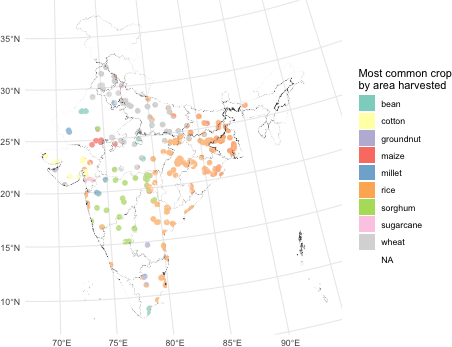
\includegraphics{draft_files/figure-latex/crops-1} \caption[Most common crop by village]{Most common crop by village}\label{fig:crops}\floatfoot*{Note: The figure shows the most common crop grown in each village, by area harvested.}
\end{figure}

\hypertarget{crops-and-labor-intensity}{%
\subsection{Crops and labor intensity}\label{crops-and-labor-intensity}}

A key question about the results is the mechanism. While previous results indicate that pollution may actually increase land productivity (Sanders and Barreca 2022), the results in that paper come from the United States, where agricultural practices vary greatly from those in India. On the other hand, we also know that pollution can affect labor productivity in other contexts (Chang et al. 2019; Ebenstein, Lavy, and Roth 2016; Graff Zivin and Neidell 2012; Wen and Burke 2022). Unfortunately, there is no available labor data that would allow me to directly test the effects of pollution on agricultural labor productivity. While the National Sample Survey is nationally representative, it does not allow one to back out productivity, only total labor allocation in the preceding week. Additional data options -- like the ARIS-REDS or IHDS -- are not collected frequently enough to enable the kind of analysis employed here.

Instead, I look at heterogeneity by the modal crop grown in each area. I use data from Monfreda, Ramankutty, and Foley (2008), who estimate area harvested by crop at a resolution of approximately 10km. These estimates come from around the year 2000, at the beginning of my sample period. I identify areas where rice is the most commonly grown crop. Rice (paddy) is commonly regarded as a labor-intensive crop in India (Vollrath 2011; Michler 2020), meaning that it may be more susceptible to pollution if some of the effects of pollution are through direct effects on labor productivity.

Figure \ref{fig:crops} shows the distribution of the most common crop across the villages in my sample. Though there are large areas where rice is the most commonly grown crop, there is also quite a bit of overlap, especially in the middle parts of the country. However, given the geographic concentration of rice production, I will implement a robustness check with state-by-year fixed effects below.

\begin{table}

\caption{\label{tab:yieldrice}Agricultural productivity by most common crop}
\centering
\begin{threeparttable}
\begin{tabular}[t]{>{\raggedright\arraybackslash}p{5.5cm}>{\centering\arraybackslash}p{2cm}>{\centering\arraybackslash}p{2cm}}
\toprule
  & (1) & (2)\\
\midrule
Particulate matter (log PM 2.5) & -0.287** & -0.394***\\
 & (0.133) & (0.134)\\
PM 2.5 times rice & -0.338*** & -0.205***\\
 & (0.061) & (0.060)\\
Weather (expanded) & Yes & No\\
Weather (expanded, bins) & No & Yes\\
\textbf{Fixed effects:} & \textbf{} & \textbf{}\\
Village & Yes & Yes\\
Year & Yes & Yes\\
\midrule
F (PM 2.5) & 1,369 & 1,168\\
F (PM 2.5 times rice) & 2,107 & 2,201\\
Observations & 1,266,922 & 1,266,922\\
\bottomrule
\end{tabular}
\begin{tablenotes}[para]
\item Note: Standard errors are in parentheses and are clustered at the village level. The outcome in all regressions estimated agricultural yield (tons per hectare). The rice dummy equals one in villages where rice is the most commonly harvested crop. * p<0.10 ** p<0.05 *** p<0.01
\end{tablenotes}
\end{threeparttable}
\end{table}

Table \ref{tab:yieldrice} presents the main results in this section. I continue to employ an IV strategy, interacting pollution with an indicator for rice and instrumenting this with an interaction between wind and rice. The first row shows the effects of overall pollution on agricultural productivity in villages where rice is not the most commonly grown crop. Column two, which has the most flexible weather specification, indicates that an increase of particulate matter by one percent decreases productivity in these areas by around 0.4 percent. The second row is an interaction term between rice and PM 2.5, meaning the linear combination of the two coefficients gives the overall effect of pollution on productivity in rice-predominant villages. The coefficient of -0.2 shows that pollution decreases productivity by around 50 percent more in rice-growing villages than in non-rice growing villages. Since rice is more labor intensive, this is evidence that the effects of pollution work at least partly through the effects of pollution on labor productivity. This does not, however, rule out any direct effects on land productivity.

Given the geographic concentration of crops, Table \ref{tab:yieldricestatefe} in the appendix presents the same results but with state-by-year fixed effects, instead of just year fixed effects. This will compare the effects of pollution within states in the same year, hopefully decreasing concerns that something other than labor intensity is the main driver of the heterogeneity documented in Table \ref{tab:yieldrice}. The results are consistent with those presented here, and show that pollution decreases productivity more in rice-growing villages than in other villages.

\hypertarget{coal-plants-or-overall-pollution}{%
\subsection{Coal plants or overall pollution?}\label{coal-plants-or-overall-pollution}}

Finally, while I identify high-pollution areas using the location of coal plants, an important question is how much of the overall effect is driven by coal plants and how much is driven by other polluting industries located in areas near coal plants. I try to answer this question in Table \ref{tab:yield7ivdiffindiff}, where I implement an instrumental variables differences-in-differences, essentially instrumenting for pollution prior to the opening of a coal plant with wind and instrumenting for the interaction term (pollution times plant opening) with wind times plant opening.

Columns one and two of Table \ref{tab:yield7ivdiffindiff} present specifications with slightly different weather controls. Column two presents the most extensive set of controls -- the flexible specification with binned weather variables -- and I focus on that column here. First, there are now two first stages but the F-tests indicate that the instruments are strong for both, including the interaction term (F = 205 in the second column). Second, the first row shows the effect of pollution on agricultural productivity prior to the opening of a coal plant; the coefficient is negative, indicating negative effects of non-coal pollution. Third, the interaction term is strongly negative and approximately the same in magnitude as the level term, indicating a very clear effect specific to coal plants, in addition to the overall negative effect of pollution.

\begin{table}

\caption{\label{tab:yield7ivdiffindiff}Agricultural productivity and pollution source}
\centering
\begin{threeparttable}
\begin{tabular}[t]{>{\raggedright\arraybackslash}p{5.5cm}>{\centering\arraybackslash}p{2cm}>{\centering\arraybackslash}p{2cm}}
\toprule
  & (1) & (2)\\
\midrule
Particulate matter (log PM 2.5) & -0.228*** & -0.223***\\
 & (0.066) & (0.065)\\
PM 2.5 times Coal & -0.250*** & -0.220***\\
 & (0.024) & (0.025)\\
Weather (expanded) & Yes & No\\
Weather (expanded, bins) & No & Yes\\
\textbf{Fixed effects:} & \textbf{} & \textbf{}\\
Year & Yes & Yes\\
Village & Yes & Yes\\
\midrule
F (PM) & 769 & 772\\
F (PM times Coal) & 231 & 205\\
Observations & 1,266,922 & 1,266,922\\
\bottomrule
\end{tabular}
\begin{tablenotes}[para]
\item Note: Standard errors are in parentheses and are clustered at the village level. The outcome in all regressions is estimated agricultural yield, defined as tons per hectare. * p<0.10 ** p<0.05 *** p<0.01
\end{tablenotes}
\end{threeparttable}
\end{table}

Importantly, since these results come from an IV, both coefficients denote the change in agricultural yield due to an increase in pollution by the same units. In other words, this is not identifying differences in overall pollution, per se, but rather differences in the effects of an increase of pollution by the same percentage. These different effects could be due to, for example, differences in emission patterns for different kinds of plants and factories; coal plants, for example, are responsible for much more mercury than other kinds of polluting industries.\footnote{\url{https://www.epa.gov/sites/default/files/2016-12/documents/nei2014v1_tsd.pdf}}

\hypertarget{conclusion}{%
\section{Conclusion}\label{conclusion}}

\label{conclusion}

In this paper, I show some of the negative effects associated with pollution, in general, and coal pollution, in particular. Using exogenous variation in pollution driven by changes in wind direction, results here show that pollution has a large, negative effect on agricultural productivity in India. These negative effects are at least partly due to changes in labor productivity; areas growing more labor-intensive crops see larger decreases in agricultural productivity due to pollution. Nonetheless, I am unable to rule out direct effects on land productivity with the data available.

Using instrumental variables in a differences-in-differences set up, I also show that the effects of pollution from coal, in particular, are particularly harmful to agricultural productivity. Changes of an equivalent increase in pollution lead to three times larger negative effects on agricultural productivity following the opening of a coal plant, compared to just before.

These results document relatively large, local externalities in the agricultural sector in a developing country. Since the sector is a refuge for some of the poorest citizens in the world, the results raise important questions about the current speed of the energy transition as it relates to sustainable development and poverty reduction, more generally. While we often frame the debate around greenhouse gasses in terms of climate change, there are important local reasons to reduce pollution emissions, as well. The technology for greener energy exists; at this point, it is simply a question of policies (Markard 2018; Blazquez, Fuentes, and Manzano 2020).

These results, of course, do not address possible positive effects of the building of additional power plants, which can lead to increased electricity access, or shifting more of the population into non-agricultural sectors, which can raise standards of living. As such, the main conclusion is that the location of pollution emissions -- especially from coal plants -- may be particularly important for multiple aspects of economic activity, not just health and mortality.

\FloatBarrier
\newpage
\singlespacing

\hypertarget{references}{%
\section*{References}\label{references}}
\addcontentsline{toc}{section}{References}

\hypertarget{refs}{}
\begin{CSLReferences}{1}{0}
\leavevmode\vadjust pre{\hypertarget{ref-abadie2023should}{}}%
Abadie, Alberto, Susan Athey, Guido W Imbens, and Jeffrey M Wooldridge. 2023. {``When Should You Adjust Standard Errors for Clustering?''} \emph{{The Quarterly Journal of Economics}} 138 (1): 1--35.

\leavevmode\vadjust pre{\hypertarget{ref-abay2022nonclassical}{}}%
Abay, Kibrom A, Christopher B Barrett, Talip Kilic, Heather Moylan, John Ilukor, and Wilbert Drazi Vundru. 2022. {``{Nonclassical Measurement Error and Farmers' Response to Information Reveal Behavioral Anomalies}.''}

\leavevmode\vadjust pre{\hypertarget{ref-aragon2016polluting}{}}%
Aragón, Fernando M, and Juan Pablo Rud. 2016. {``{Polluting industries and agricultural productivity: Evidence from mining in Ghana}.''} \emph{{The Economic Journal}} 126 (597): 1980--2011.

\leavevmode\vadjust pre{\hypertarget{ref-almn2021}{}}%
Asher, Sam, Tobias Lunt, Ryu Matsuura, and Paul Novosad. 2021. {``{Development Research at High Geographic Resolution: An Analysis of Night Lights, Firms, and Poverty in India using the SHRUG Open Data Platform}.''} \emph{{The World Bank Economic Review}}.

\leavevmode\vadjust pre{\hypertarget{ref-barrios2012clustering}{}}%
Barrios, Thomas, Rebecca Diamond, Guido W Imbens, and Michal Kolesár. 2012. {``Clustering, Spatial Correlations, and Randomization Inference.''} \emph{{Journal of the American Statistical Association}} 107 (498): 578--91.

\leavevmode\vadjust pre{\hypertarget{ref-bencko1977health}{}}%
Bencko, Vladimir, and Karel Symon. 1977. {``Health Aspects of Burning Coal with a High Arsenic Content.''} \emph{{Environmental Research}} 13 (3): 378--85.

\leavevmode\vadjust pre{\hypertarget{ref-bertrand2004much}{}}%
Bertrand, Marianne, Esther Duflo, and Sendhil Mullainathan. 2004. {``How Much Should We Trust Differences-in-Differences Estimates?''} \emph{{The Quarterly Journal of Economics}} 119 (1): 249--75.

\leavevmode\vadjust pre{\hypertarget{ref-blazquez2020some}{}}%
Blazquez, Jorge, Rolando Fuentes, and Baltasar Manzano. 2020. {``On Some Economic Principles of the Energy Transition.''} \emph{{Energy Policy}} 147: 111807.

\leavevmode\vadjust pre{\hypertarget{ref-borgschulte2022air}{}}%
Borgschulte, Mark, David Molitor, and Eric Yongchen Zou. 2022. {``{Air pollution and the labor market: Evidence from wildfire smoke}.''} \emph{{Review of Economics and Statistics}}, 1--46.

\leavevmode\vadjust pre{\hypertarget{ref-burney2014recent}{}}%
Burney, Jennifer, and V Ramanathan. 2014. {``{Recent climate and air pollution impacts on Indian agriculture}.''} \emph{{Proceedings of the National Academy of Sciences}} 111 (46): 16319--24.

\leavevmode\vadjust pre{\hypertarget{ref-chang2019effect}{}}%
Chang, Tom Y, Joshua Graff Zivin, Tal Gross, and Matthew Neidell. 2019. {``{The effect of pollution on worker productivity: evidence from call center workers in China}.''} \emph{{American Economic Journal: Applied Economics}} 11 (1): 151--72.

\leavevmode\vadjust pre{\hypertarget{ref-chen2022effect}{}}%
Chen, Shuai, Paulina Oliva, and Peng Zhang. 2022. {``{The effect of air pollution on migration: evidence from China}.''} \emph{{Journal of Development Economics}} 156: 102833.

\leavevmode\vadjust pre{\hypertarget{ref-christiaensen2011evolving}{}}%
Christiaensen, Luc, Lionel Demery, and Jesper Kuhl. 2011. {``{The (evolving) role of agriculture in poverty reduction --- An empirical perspective}.''} \emph{{Journal of Development Economics}} 96 (2): 239--54.

\leavevmode\vadjust pre{\hypertarget{ref-dercon2002income}{}}%
Dercon, Stefan. 2002. {``Income Risk, Coping Strategies, and Safety Nets.''} \emph{{The World Bank Research Observer}} 17 (2): 141--66.

\leavevmode\vadjust pre{\hypertarget{ref-dercon2009rural}{}}%
---------. 2009. {``{Rural poverty: Old challenges in new contexts}.''} \emph{{The World Bank Research Observer}} 24 (1): 1--28.

\leavevmode\vadjust pre{\hypertarget{ref-deryugina2019mortality}{}}%
Deryugina, Tatyana, Garth Heutel, Nolan H Miller, David Molitor, and Julian Reif. 2019. {``{The mortality and medical costs of air pollution: Evidence from changes in wind direction}.''} \emph{{American Economic Review}} 109 (12): 4178--4219.

\leavevmode\vadjust pre{\hypertarget{ref-desiere2018land}{}}%
Desiere, Sam, and Dean Jolliffe. 2018. {``{Land productivity and plot size: Is measurement error driving the inverse relationship?}''} \emph{{Journal of Development Economics}} 130: 84--98.

\leavevmode\vadjust pre{\hypertarget{ref-dinkelman2011effects}{}}%
Dinkelman, Taryn. 2011. {``{The effects of rural electrification on employment: New evidence from South Africa}.''} \emph{{American Economic Review}} 101 (7): 3078--108.

\leavevmode\vadjust pre{\hypertarget{ref-ebenstein2016long}{}}%
Ebenstein, Avraham, Victor Lavy, and Sefi Roth. 2016. {``{The long-run economic consequences of high-stakes examinations: Evidence from transitory variation in pollution}.''} \emph{{American Economic Journal: Applied Economics}} 8 (4): 36--65.

\leavevmode\vadjust pre{\hypertarget{ref-gangopadhyay2022new}{}}%
Gangopadhyay, Prasun K, Paresh B Shirsath, Vinay K Dadhwal, and Pramod K Aggarwal. 2022. {``{A new two-decade (2001--2019) high-resolution agricultural primary productivity dataset for India}.''} \emph{{Scientific Data}} 9 (1): 1--12.

\leavevmode\vadjust pre{\hypertarget{ref-gillen2019experimenting}{}}%
Gillen, Ben, Erik Snowberg, and Leeat Yariv. 2019. {``{Experimenting with measurement error: Techniques with applications to the Caltech cohort study}.''} \emph{{Journal of Political Economy}} 127 (4): 1826--63.

\leavevmode\vadjust pre{\hypertarget{ref-glewwe2012much}{}}%
Glewwe, Paul. 2012. {``{How much of observed economic mobility is measurement error? IV methods to reduce measurement error bias, with an application to Vietnam}.''} \emph{{The World Bank Economic Review}} 26 (2): 236--64.

\leavevmode\vadjust pre{\hypertarget{ref-graff2012impact}{}}%
Graff Zivin, Joshua, and Matthew Neidell. 2012. {``{The impact of pollution on worker productivity}.''} \emph{{American Economic Review}} 102 (7): 3652--73.

\leavevmode\vadjust pre{\hypertarget{ref-hammer2020global}{}}%
Hammer, Melanie S, Aaron van Donkelaar, Chi Li, Alexei Lyapustin, Andrew M Sayer, N Christina Hsu, Robert C Levy, et al. 2020. {``Global Estimates and Long-Term Trends of Fine Particulate Matter Concentrations (1998--2018).''} \emph{{Environmental Science \& Technology}} 54 (13): 7879--90.

\leavevmode\vadjust pre{\hypertarget{ref-hanna2015effect}{}}%
Hanna, Rema, and Paulina Oliva. 2015. {``{The effect of pollution on labor supply: Evidence from a natural experiment in Mexico City}.''} \emph{{Journal of Public Economics}} 122: 68--79.

\leavevmode\vadjust pre{\hypertarget{ref-he2019severe}{}}%
He, Jiaxiu, Haoming Liu, and Alberto Salvo. 2019. {``{Severe air pollution and labor productivity: Evidence from industrial towns in China}.''} \emph{{American Economic Journal: Applied Economics}} 11 (1): 173--201.

\leavevmode\vadjust pre{\hypertarget{ref-heck1982assessment}{}}%
Heck, Walter W, OC Taylor, Richard Adams, Gail Bingham, Joseph Miller, Eric Preston, and Leonard Weinstein. 1982. {``{Assessment of crop loss from ozone}.''} \emph{{Journal of the Air Pollution Control Association}} 32 (4): 353--61.

\leavevmode\vadjust pre{\hypertarget{ref-herrendorf2014growth}{}}%
Herrendorf, Berthold, Richard Rogerson, and Akos Valentinyi. 2014. {``Growth and Structural Transformation.''} \emph{{Handbook of Economic Growth}} 2: 855--941.

\leavevmode\vadjust pre{\hypertarget{ref-kline2014local}{}}%
Kline, Patrick, and Enrico Moretti. 2014. {``{Local economic development, agglomeration economies, and the big push: 100 years of evidence from the Tennessee Valley Authority}.''} \emph{The Quarterly Journal of Economics} 129 (1): 275--331.

\leavevmode\vadjust pre{\hypertarget{ref-kopas2020environmental}{}}%
Kopas, Jacob, Erin York, Xiaomeng Jin, SP Harish, Ryan Kennedy, Shiran Victoria Shen, and Johannes Urpelainen. 2020. {``{Environmental justice in India: incidence of air pollution from coal-fired power plants}.''} \emph{{Ecological Economics}} 176: 106711.

\leavevmode\vadjust pre{\hypertarget{ref-lee2022valid}{}}%
Lee, David, Justin McCrary, Marcelo J Moreira, and Jack Porter. 2022. {``{Valid t-ratio Inference for IV}.''} \emph{{American Economic Review}} 112 (10): 3260--90.

\leavevmode\vadjust pre{\hypertarget{ref-lee2020does}{}}%
Lee, Kenneth, Edward Miguel, and Catherine Wolfram. 2020. {``Does Household Electrification Supercharge Economic Development?''} \emph{{Journal of Economic Perspectives}} 34 (1): 122--44.

\leavevmode\vadjust pre{\hypertarget{ref-li2014health}{}}%
Li, Ya-Ru, and Jacqueline MacDonald Gibson. 2014. {``{Health and air quality benefits of policies to reduce coal-fired power plant emissions: a case study in North Carolina}.''} \emph{{Environmental Science \& Technology}} 48 (17): 10019--27.

\leavevmode\vadjust pre{\hypertarget{ref-markard2018next}{}}%
Markard, Jochen. 2018. {``The Next Phase of the Energy Transition and Its Implications for Research and Policy.''} \emph{{Nature Energy}} 3 (8): 628--33.

\leavevmode\vadjust pre{\hypertarget{ref-marshall1997hidden}{}}%
Marshall, Fiona, Mike Ashmore, Fiona Hinchcliffe, et al. 1997. \emph{{A hidden threat to food production: Air pollution and agriculture in the developing world}}. {International Institute for Environment and Development.}

\leavevmode\vadjust pre{\hypertarget{ref-merfeld2023poverty}{}}%
Merfeld, Joshua D, and Jonathan Morduch. 2023. {``Poverty at Higher Frequency.''} \emph{{KDI School of Pub Policy \& Management Paper No. DP23-03}}.

\leavevmode\vadjust pre{\hypertarget{ref-michler2020agriculture}{}}%
Michler, Jeffrey D. 2020. {``{Agriculture in the process of development: A micro-perspective}.''} \emph{{World Development}} 129: 104888.

\leavevmode\vadjust pre{\hypertarget{ref-monfreda2008farming}{}}%
Monfreda, Chad, Navin Ramankutty, and Jonathan A Foley. 2008. {``{Farming the planet: Geographic distribution of crop areas, yields, physiological types, and net primary production in the year 2000}.''} \emph{{Global Biogeochemical Cycles}} 22 (1).

\leavevmode\vadjust pre{\hypertarget{ref-ramanathan2008global}{}}%
Ramanathan, Veerabhadran, and Gregory Carmichael. 2008. {``{Global and regional climate changes due to black carbon}.''} \emph{{Nature Geoscience}} 1 (4): 221--27.

\leavevmode\vadjust pre{\hypertarget{ref-reddy2006impact}{}}%
Reddy, V Ratna, and Bhagirath Behera. 2006. {``{Impact of water pollution on rural communities: An economic analysis}.''} \emph{{Ecological Economics}} 58 (3): 520--37.

\leavevmode\vadjust pre{\hypertarget{ref-rud2012electricity}{}}%
Rud, Juan Pablo. 2012. {``{Electricity provision and industrial development: Evidence from India}.''} \emph{{Journal of Development Economics}} 97 (2): 352--67.

\leavevmode\vadjust pre{\hypertarget{ref-sanders2022adaptation}{}}%
Sanders, Nicholas J, and Alan I Barreca. 2022. {``{Adaptation to Environmental Change: Agriculture and the Unexpected Incidence of the Acid Rain Program}.''} \emph{{American Economic Journal: Economic Policy}} 14 (1): 373--401.

\leavevmode\vadjust pre{\hypertarget{ref-van2017long}{}}%
Van de Walle, Dominique, Martin Ravallion, Vibhuti Mendiratta, and Gayatri Koolwal. 2017. {``{Long-term gains from electrification in rural India}.''} \emph{{The World Bank Economic Review}} 31 (2): 385--411.

\leavevmode\vadjust pre{\hypertarget{ref-vollrath2011agricultural}{}}%
Vollrath, Dietrich. 2011. {``The Agricultural Basis of Comparative Development.''} \emph{{Journal of Economic Growth}} 16: 343--70.

\leavevmode\vadjust pre{\hypertarget{ref-wen2022lower}{}}%
Wen, Jeff, and Marshall Burke. 2022. {``{Lower test scores from wildfire smoke exposure}.''} \emph{{Nature Sustainability}} 5 (11): 947--55.

\end{CSLReferences}

\FloatBarrier
\newpage

\hypertarget{appendix-a}{%
\section*{Appendix A}\label{appendix-a}}
\addcontentsline{toc}{section}{Appendix A}

\beginappendix
\FloatBarrier

\begin{table}[H]

\caption{\label{tab:data}Data sources}
\centering
\begin{threeparttable}
\begin{tabular}[t]{>{\raggedright\arraybackslash}p{2cm}>{\centering\arraybackslash}p{5cm}>{\centering\arraybackslash}p{3cm}>{\centering\arraybackslash}p{3cm}}
\toprule
  & source & geographic coverage & temporal coverage\\
\midrule
shapefile & Asher et al. (2021) & India & \\
coal plants & Global Energy Monitor & global & yearly\\
wind & NCAR & global & daily\\
pollution & Hammer et al. (2020) & global & monthly\\
agriculture & Gangopadhya et al. (2022) & India & two seasons/year\\
weather & TerraClimate & global & monthly\\
crops & Monfreda et al. (2008) & global & 2000 (year)\\
\bottomrule
\end{tabular}
\begin{tablenotes}[para]
\item Global Energy Monitor: globalenergymonitor.org/projects/global-coal-plant-tracker. NCAR: climatedataguide.ucar.edu/. TerraClimate: www.climatologylab.org/terraclimate.html
\end{tablenotes}
\end{threeparttable}
\end{table}

\FloatBarrier
\newpage

\begin{figure}
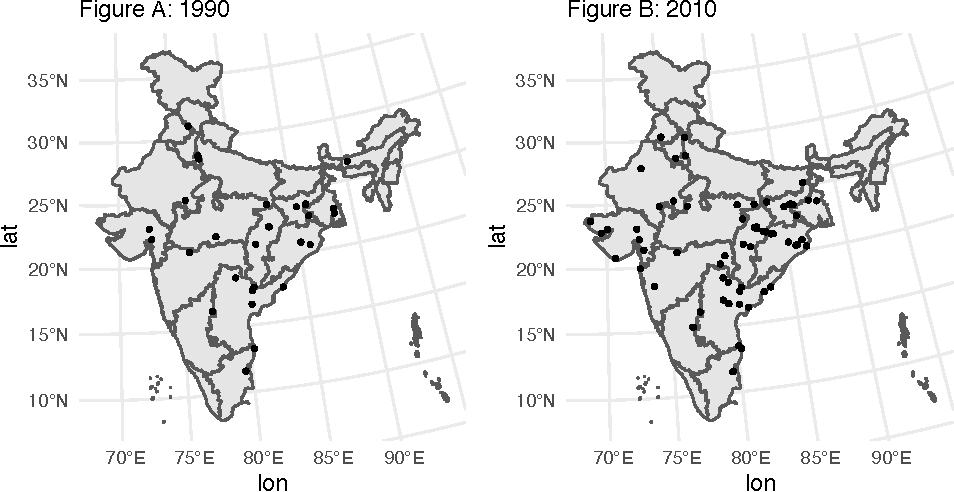
\includegraphics{draft_files/figure-latex/plants-1} \caption[Coal plants in India from 1990 to 2010]{Coal plants in India from 1990 to 2010}\label{fig:plants}\floatfoot*{Note: The left figure shows the location of coal plants of at least 30MW in 1990. The right figure shows the location of such coal plants in 2010.}
\end{figure}

\FloatBarrier
\newpage

\begin{figure}
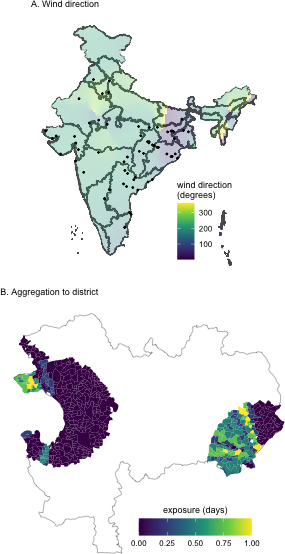
\includegraphics{draft_files/figure-latex/windexample-1} \caption[Wind direction and aggregation examples (2010-01-01)]{Wind direction and aggregation examples (2010-01-01)}\label{fig:windexample}\floatfoot*{Note: The top figure shows the average wind direction on January 1st, 2010, with zero degrees indicating north. The points are the location of coal plants on that date. The bottom figure shows the distribution of pollution exposure in a specific district -- Guna district in Madhya Pradesh -- on the same date.}
\end{figure}

\FloatBarrier
\newpage

\begin{table}

\caption{\label{tab:yield3ivmainfirststage}Wind direction and particulate matter}
\centering
\begin{threeparttable}
\begin{tabular}[t]{>{\raggedright\arraybackslash}p{4cm}>{\centering\arraybackslash}p{2cm}>{\centering\arraybackslash}p{2cm}>{\centering\arraybackslash}p{2cm}>{\centering\arraybackslash}p{2cm}}
\toprule
  & (1) & (2) & (3) & (4)\\
\midrule
wind & 0.0083*** & 0.0085*** & 0.0083*** & 0.0085***\\
 & (0.0002) & (0.0002) & (0.0002) & (0.0002)\\
weather & No & Yes & Yes & No\\
weather (expanded) & No & No & Yes & No\\
weather (expanded, bins) & No & No & No & Yes\\
\textbf{fixed effects:} & \textbf{} & \textbf{} & \textbf{} & \textbf{}\\
village & Yes & Yes & Yes & Yes\\
year & Yes & Yes & Yes & Yes\\
\midrule
F & 1,236 & 1,266 & 1,205 & 1,246\\
observations & 1,266,922 & 1,266,922 & 1,266,922 & 1,266,922\\
\bottomrule
\end{tabular}
\begin{tablenotes}[para]
\item Note: Standard errors are in parentheses and are clustered at the village level. * p<0.10 ** p<0.05 *** p<0.01
\end{tablenotes}
\end{threeparttable}
\end{table}

\FloatBarrier
\newpage

\begin{figure}
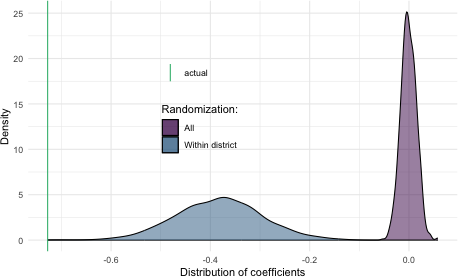
\includegraphics{draft_files/figure-latex/randomplot-1} \caption[Randomization inference]{Randomization inference}\label{fig:randomplot}\floatfoot*{Note: The figure presents the distribution of coefficients by randomly assigning wind direction across villages within the same year. The "all" distribution is created by randomly assigning a single wind value to each village, sampled with replacement across all villages in a given year. The "within district" randomly samples with replacement only from within the same district in the same year.}
\end{figure}

\FloatBarrier
\newpage

\FloatBarrier
\newpage

\begin{table}

\caption{\label{tab:yield8cumulative}Cumulative exposure to pollution during the season}
\centering
\begin{threeparttable}
\begin{tabular}[t]{>{\raggedright\arraybackslash}p{2.25cm}>{\centering\arraybackslash}p{2cm}>{\centering\arraybackslash}p{2cm}>{\centering\arraybackslash}p{2cm}>{\centering\arraybackslash}p{2cm}>{\centering\arraybackslash}p{2cm}}
\toprule
  & (1) & (2) & (3) & (4) & (5)\\
\midrule
June & -0.643*** &  &  &  & \\
 & (0.064) &  &  &  & \\
July &  & -0.658*** &  &  & \\
 &  & (0.045) &  &  & \\
Aug. &  &  & -0.531*** &  & \\
 &  &  & (0.049) &  & \\
Sept. &  &  &  & -0.672*** & \\
 &  &  &  & (0.047) & \\
Oct. &  &  &  &  & -0.943***\\
 &  &  &  &  & (0.069)\\
weather & Yes & Yes & Yes & Yes & Yes\\
\textbf{fixed effects:} & \textbf{} & \textbf{} & \textbf{} & \textbf{} & \textbf{}\\
village & Yes & Yes & Yes & Yes & Yes\\
year & Yes & Yes & Yes & Yes & Yes\\
\midrule
F & 1,327 & 2,830 & 2,933 & 2,413 & 1,515\\
observations & 1,266,922 & 1,266,922 & 1,266,922 & 1,266,922 & 1,266,922\\
\bottomrule
\end{tabular}
\begin{tablenotes}[para]
\item Note: Standard errors are in parentheses and are clustered at the village level. * p<0.10 ** p<0.05 *** p<0.01
\end{tablenotes}
\end{threeparttable}
\end{table}

\FloatBarrier
\newpage

\begin{table}

\caption{\label{tab:yieldricestatefe}Agricultural productivity by most common crop}
\centering
\begin{threeparttable}
\begin{tabular}[t]{>{\raggedright\arraybackslash}p{3.5cm}>{\centering\arraybackslash}p{2cm}>{\centering\arraybackslash}p{2cm}}
\toprule
  & (1) & (2)\\
\midrule
Particulate matter & -0.811*** & -1.034***\\
(log PM 2.5) & (0.158) & (0.144)\\
PM 2.5 times rice & -1.204*** & -0.966***\\
 & (0.095) & (0.092)\\
Weather (expanded) & Yes & No\\
Weather (expanded, bins) & No & Yes\\
\textbf{Fixed effects:} & \textbf{} & \textbf{}\\
Village & Yes & Yes\\
Year & Yes & Yes\\
\midrule
F (PM 2.5) & 883 & 941\\
F (PM 2.5 times rice) & 1,355 & 1,395\\
Observations & 1,266,922 & 1,266,922\\
\bottomrule
\end{tabular}
\begin{tablenotes}[para]
\item Note: Standard errors are in parentheses and are clustered at the village level. The outcome in all regressions estimated agricultural yield (tons per hectare). The rice dummy equals one in villages where rice is the most commonly harvested crop. * p<0.10 ** p<0.05 *** p<0.01
\end{tablenotes}
\end{threeparttable}
\end{table}

\end{document}
